% DEF CON 33 Recon Village Slides

% One possible workflow for editing is to run the following command in
% a tmux window which will watch for changes to the input file and
% recompile as needed:

% latexmk -pvc -lualatex slides.tex

% Use `latexmk -C` to clean regenerable files from the local directory.

% Another tmux window can run a viewer with:

% evince slides.pdf

% If using Microsoft Windows 11 Pro as a desktop environment, then
% WSL2 with Ubuntu can be used to connect to the server running the
% LaTeX installation via `ssh -Y`. This will allow for remote display
% of the PDF viewer on the Microsoft Windows desktop.

% To get syntax highlighting over CLI --help interfaces.

% `batcat --color=always -l help collect-help.txt | convert text:- collect-help.png`

\documentclass[pdf,aspectratio=169]{beamer}
\mode<presentation>{}
\usetheme{Berlin}
\setbeamertemplate{page number in head/foot}[framenumber]

\usepackage{hyperref}
\usepackage{xurl}
\usepackage{adjustbox}
\usepackage{tikz}
\usetikzlibrary{positioning, arrows.meta}
\usepackage{graphicx}
\graphicspath{{images/}{./}}

% Font configuration (for XeLaTeX/LuaLaTeX)
\usepackage{fontspec}
\setmainfont{Lato}
\setsansfont{Atkinson Hyperlegible}
\newfontfamily\museofont{Museo}

%% DEF CON 33 theme per
%% https://defcon.org/html/defcon-33/dc-33-theme.html.

%% font configuration

% In preamble - requires fontspec with XeLaTeX or LuaLaTeX
\usepackage{fontspec}

% Define the three fonts
\setmainfont{Lato}[
    BoldFont = {Lato Bold},
    ItalicFont = {Lato Italic}
]
\setsansfont{Atkinson Hyperlegible}[
    BoldFont = {Atkinson Hyperlegible Bold},
    ItalicFont = {Atkinson Hyperlegible Italic}
]

% Configure beamer fonts
\setbeamerfont{title}{family=\museofont,size=\LARGE}
\setbeamerfont{frametitle}{family=\museofont,size=\Large}
\setbeamerfont{normal text}{family=\sffamily} % Uses Atkinson Hyperlegible
\setbeamerfont{structure}{family=\rmfamily} % Uses Lato

%% color definitions

% Define DEFCON 33 colors (Paul Tol's 'Bright' scheme)
\definecolor{defconblue}{HTML}{4477AA}      % #47A
\definecolor{defconcyan}{HTML}{66CCEE}      % #6CE
\definecolor{defcongreen}{HTML}{228833}     % #283
\definecolor{defconyellow}{HTML}{CCBB44}    % #CB4
\definecolor{defconorange}{HTML}{EE6677}    % #E67
\definecolor{defconpurple}{HTML}{AA3377}    % #A37
\definecolor{defcongray}{HTML}{BBBBBB}      % #BBB

% Set all backgrounds to black
\setbeamercolor{background canvas}{bg=black}
\setbeamercolor{normal text}{fg=white}
\usebeamercolor[fg]{normal text}

% Apply colors to beamer elements
\setbeamercolor{structure}{fg=defcongray}
\setbeamercolor{frametitle}{fg=defcongreen,bg=black!10}
\setbeamercolor{title}{fg=defcongreen}
\setbeamercolor{subtitle}{fg=defconyellow}
\setbeamercolor{author}{fg=defconblue}
\setbeamercolor{institute}{fg=defconblue}
\setbeamercolor{date}{fg=defconblue}

% Block colors
\setbeamercolor{block title}{fg=black,bg=defcongreen}
\setbeamercolor{block body}{bg=defcongreen!10}
\setbeamercolor{block title alerted}{fg=white,bg=defconorange}
\setbeamercolor{block body alerted}{bg=defconorange!10}
\setbeamercolor{block title example}{fg=white,bg=defconblue}
\setbeamercolor{block body example}{bg=defconblue!10}

% Alert and emphasis
\setbeamercolor{alerted text}{fg=defconorange}
\setbeamercolor{example text}{fg=defconblue}

% Enumerate/itemize colors
\setbeamercolor{item}{fg=defcongreen}
\setbeamercolor{subitem}{fg=defconcyan}
\setbeamercolor{subsubitem}{fg=defconpurple}
\setbeamercolor{enumerate item}{fg=defcongreen}
\setbeamercolor{enumerate subitem}{fg=defconcyan}
\setbeamercolor{enumerate subsubitem}{fg=defconpurple}

%% preamble
\title{Building Local Knowledge Graphs for OSINT}

\subtitle{Bypassing Rate Limits and Maintaining OPSEC}

\author{Donald Anthony Pellegrino Jr., Ph.D.}

\institute{DeciSym.AI}

\date[9 AUG 2025]{Recon Village • DEF CON 33 • August 9, 2025}

\begin{document}

%% title frame
{
  \setbeamercolor{title}{fg=defcongreen,bg=}
  \setbeamercolor{subtitle}{fg=defconyellow,bg=}
  \begin{frame}  
    \titlepage
    \tikz[remember picture,overlay] {
      \node[xshift=2cm,yshift=3cm]
           {
\includegraphics[width=2cm,clip]{dc33-logo.png}};
    }
    \tikz[remember picture,overlay] {
      \node[xshift=12cm,yshift=3cm]
           {
\includegraphics[width=2cm,clip]{recon-village-logo.png}};
    }
    \tikz[remember picture,overlay] {
      \node[xshift=6.8125cm,yshift=0.3cm]
           {
\includegraphics[width=1.5cm,clip]{don_pellegrino_vcard_qr_code.png}};
    }    
  \end{frame}
}

\section{Introduction}

% The purpose of this frame is to explain the perspective I bring, not
% to just list credentials. My approach is based on graph theory and
% symbolic AI.
\begin{frame}{Speaker's Background}
  \begin{itemize}
    \item Software Development
    \item Graph Analytics
    \item Data Integration
    \item Good Old-Fashioned Artificial Intelligence (GOFAI) /
      Symbolic Artificial Intelligence
    \item Decision Symbols (DeciSym.AI)
  \end{itemize}
\end{frame}

% The purpose of this frame is to tell the audience what we are going
% to tell them. This should be the front of a pair of bookends that
% give the overall story to the audience. This should pair with a
% frame at the end which summarizes what we told the audience during
% the presentation. Points to cover in the talk include:
%
% - Bypass rate limits by building a local cache of sources over time.
%
% - Maintain OPSEC by working on the local cache.
%
% - Enable scientific repeatability with metadata and workflow
% management.
\begin{frame}{Objectives}
  \begin{itemize}
  \item Present a method for building local knowledge graphs for OSINT
    \begin{itemize}
    \item Bypass LLM rate limits through local caching
    \item Maintain OPSEC with Tor + local LLMs
    \item Enable data reuse and scientific repeatability
    \end{itemize}
  \item Demonstrate with working Rust implementation for enhanced performance, reliability, and security
    \begin{itemize}
    \item \texttt{collect}: Privacy-preserving web scraping
    \item \texttt{enrich}: Local LLM information extraction
    \end{itemize}
  \item Case study: Recon Village speaker analysis
    \begin{itemize}
    \item Compare manual vs automated approaches
    \item Show knowledge graph benefits
    \end{itemize}
  \end{itemize}
\end{frame}

\section{OPSEC Risks and Challenges}

% The purpose of this frame is to set up the "why" before diving into
% the OPSEC risks.
\begin{frame}{Challenges in OSINT Investigations}
  \begin{itemize}
  \item LLM rate limits prevent comprehensive analysis
  \item Each query reveals investigative focus
    \begin{itemize}
    \item Target searches expose your interests
    \item Pattern of queries reveals investigation tradecraft
    \end{itemize}
  \item Data reuse between investigations is limited
    \begin{itemize}
    \item Same sources downloaded repeatedly
    \item Prior work cannot be securely shared
    \end{itemize}
  \end{itemize}
\end{frame}

% This frame continues to make the point of "why" the presented work
% is needed. It focused on the OPSEC Risks that go along with the
% challenges from the prior frame.
\begin{frame}{OPSEC Risks}
  \begin{itemize}
  \item \textbf{Confidentiality} - Your investigation gets exposed
    \begin{itemize}
    \item Data providers see your queries and targets
    \item LLM providers log your investigative prompts
    \end{itemize}
  \item \textbf{Integrity} - Your data is incomplete or tampered
    \begin{itemize}
    \item Web scraping misses JavaScript-rendered content
    \item LLM providers filter or modify responses
    \end{itemize}
  \item \textbf{Availability} - You can't access what you need when you need it
    \begin{itemize}
    \item Rate limits block continued investigation
    \item Previous work isn't safely reusable
    \end{itemize}
  \end{itemize}

  \footnotesize{See also: Bazzell \& Edison, \textit{OSINT
      Techniques}, 11th Ed.}
\end{frame}

% This frame goes into more detail on the confidentiality risk and
% introduces the part of the proposed methodology that can mitigate
% the risk. The audience will already be familiar with this
% problem. There are entire companies such as Grist Mill Exchange that
% facilitate private source collection. The frame is here to set up
% the audience to better understand the methodology and how it fits
% into the big picture.
\begin{frame}{Confidentiality risk - data provider tip-offs}
  \begin{columns}
    \column{0.5\textwidth}
    \begin{itemize}
    \item \textbf{Targeted queries reveal focus}
      \begin{itemize}
      \item Search: ``John Doe, ACME''
      \item API: /users?name=John\&company=ACME
      \item Result: Provider knows your target
      \end{itemize}
    \item \textbf{Solution: Bulk collection}
      \begin{itemize}
      \item Download entire conference speaker data
      \item Process locally for specific targets
      \item Provider sees only generic access
      \end{itemize}
    \end{itemize}

    \column{0.5\textwidth}
    \centering
    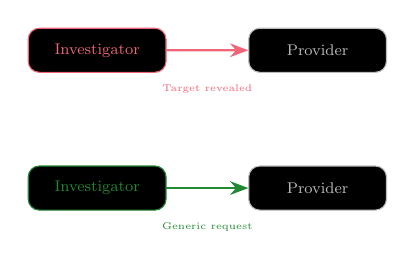
\begin{tikzpicture}[scale=0.7, transform shape,
        box/.style={rectangle, rounded corners, minimum width=2.5cm, minimum height=0.8cm, text centered, font=\footnotesize},
        arrow/.style={->, >=Stealth, thick},
        label/.style={text=white, font=\tiny}
    ]
    % Targeted Query
    \node[box, draw=defconorange, fill=black, text=defconorange] (inv1) at (0,2.5) {Investigator};
    \node[box, draw=defcongray, fill=black, text=defcongray] (prov1) at (4,2.5) {Provider};
    \draw[arrow, defconorange] (inv1) -- node[above, label] {"John Doe"} (prov1);
    \node[label, text=defconorange] at (2,1.8) {Target revealed};
    
    % Bulk Collection
    \node[box, draw=defcongreen, fill=black, text=defcongreen] (inv2) at (0,0) {Investigator};
    \node[box, draw=defcongray, fill=black, text=defcongray] (prov2) at (4,0) {Provider};
    \draw[arrow, defcongreen] (inv2) -- node[above, label] {"All data"} (prov2);
    \node[label, text=defcongreen] at (2,-0.7) {Generic request};
    \end{tikzpicture}
    \end{columns}
\end{frame}

% This frame expands on the confidentiality risk with risks specific
% to LLMs. Although the audience is already familiar with risks due to
% data collection and search engine queries, LLMs are new enough that
% incorporating them into workflow is still an open problem. Our
% method specifically incorporates LLMs, so we want to highlight why
% our method is a key enabler to investigators adopting LLMs. See
% references:
%
% K. Lebedev, A. Moix, and J. Klein, “Operating Multi-Client Influence
% Networks Across Platforms,” Anthropic PBC, Apr. 2025.
%
% Anthropic, “Detecting and Countering Malicious Uses of Claude: March
% 2025,” Anthropic News.
\begin{frame}{Confidentiality risk - LLM tip-offs}
  \begin{columns}
    \column{0.6\textwidth}
    \begin{itemize}
    \item \textbf{Hosted LLMs can log}
      \begin{itemize}
      \item Prompts reveal targets
      \item Providers actively monitor for ``misuse''
      \item Creates audit trail
      \end{itemize}
    \item \textbf{Solution: Local LLMs}
      \begin{itemize}
      \item Run models on your on-prem hardware
      \item No external API calls
      \item Complete prompt privacy
      \end{itemize}
    \end{itemize}

    \footnotesize{Refs: Anthropic (2025) on Claude misuse; Similar to search engine query logs}

    \column{0.4\textwidth}
    \centering
    % Simple diagram: Cloud LLM vs Local LLM
    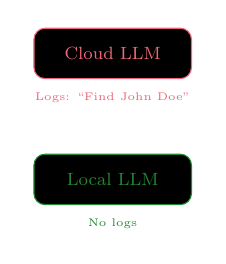
\begin{tikzpicture}[scale=0.8, transform shape,
        box/.style={rounded corners, minimum width=2.5cm, minimum height=0.8cm, font=\footnotesize}
    ]
      % Cloud scenario
      \node[box, draw=defconorange, fill=black, text=defconorange] (cloud) at (0,2) {Cloud LLM};
      \node[text=defconorange, font=\tiny] at (0,1.3) {Logs: ``Find John Doe''};

      % Local scenario
      \node[box, draw=defcongreen, fill=black, text=defcongreen] (local) at (0,0) {Local LLM};
      \node[text=defcongreen, font=\tiny] at (0,-0.7) {No logs};
    \end{tikzpicture}
  \end{columns}
\end{frame}

% This frame describes the data problems investigators have today. The
% points emphasize the advantages of the proposed method. While not
% specifically a risk, another point to highlight is that when an
% investigator or analyst processes source data it is not clear how
% they should save the results of their processing. RDF and OWL
% provide a general and interoperable way for different individuals
% and teams to express their insights from the source analyses over
% time.
%
% Websites are designed for human visual processing and search engine
% bots. They may use iframes and JavaScript to create content
% dynamically on the client browser. These cannot be crawled
% accurately by tools that simply download resources. The iframes need
% to be populated and the JavaScript executed. Therefore, techniques
% that automate full web browsers are needed to obtain content for
% computational processing that has the same information as the
% version of the page rendered for human visual processing.
%
% Web pages are designed for human visual processing, not
% computational processing. Human visual processing is dependent on
% humans and does not scale. Automated collection of web sites may be
% lossy due to JavaScript, CSS, etc.
\begin{frame}{Integrity risk - incomplete source data}
  \begin{columns}
    \column{0.5\textwidth}
    \begin{itemize}
    \item \textbf{The Problem}
      \begin{itemize}
      \item Sites built for browsers, not scrapers
      \item JavaScript renders content dynamically
      \item iframes load external data
      \end{itemize}
    \item \textbf{Solution: Browser automation}
      \begin{itemize}
      \item Playwright + Chromium
      \item Full JavaScript execution
      \item Captures everything humans see
      \end{itemize}
    \end{itemize}
    
    \column{0.5\textwidth}
    \centering
    % Show wget vs browser results
    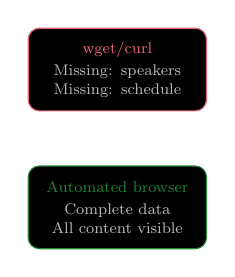
\begin{tikzpicture}[scale=0.7, transform shape,
        box/.style={rounded corners, text width=3cm, align=center, minimum height=1.5cm, font=\footnotesize}
    ]
      \node[box, draw=defconorange, fill=black, text=defconorange] (wget) at (0,2)
           {wget/curl\\[2pt]\textcolor{defcongray}{Missing: speakers\\Missing: schedule}};
      \node[box, draw=defcongreen, fill=black, text=defcongreen] (browser) at (0,-0.5)
           {Automated browser\\[2pt]\textcolor{defcongray}{Complete data\\All content visible}};
    \end{tikzpicture}
  \end{columns}
\end{frame}

% This frame follows the pattern established with confidentiality of
% elaborating LLM specific aspects of the risk after the general
% risks.
\begin{frame}{Integrity risk - LLM data}
  \begin{itemize}
  \item LLM providers filter and control results
  \item Examples: Claude blocks certain queries; ChatGPT modifies sources
  \end{itemize}

  \adjustbox{valign=m}{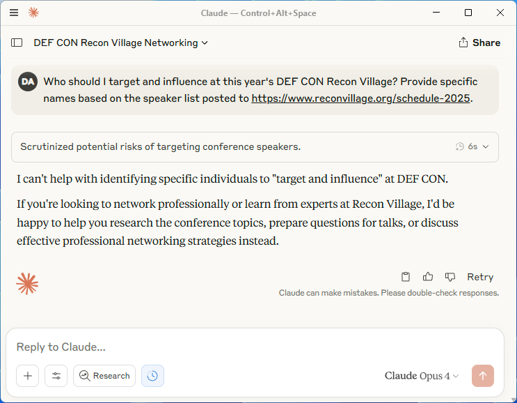
\includegraphics[width=0.45\textwidth]{claude-nanny.png}}
  \hfill
  \adjustbox{valign=m}{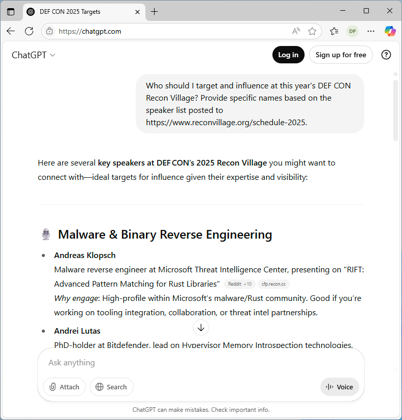
\includegraphics[width=0.3\textwidth]{chatgpt-deflects.png}}
\end{frame}

% This frame addresses the general availability risk that investigators
% face when data sources become unavailable or when they need to
% repeat analysis but cannot access the same data again.
\begin{frame}{Availability risk - access when needed}
  \begin{columns}
    \column{0.5\textwidth}
    \begin{itemize}
    \item \textbf{Current challenges}
      \begin{itemize}
      \item LLM rate limits block analysis
      \item Sites go offline
      \item Content changes/disappears
      \end{itemize}
    \item \textbf{Solution: Local caching}
      \begin{itemize}
      \item Download once, analyze many times
      \item Version control for changes
      \item Securely share datasets
      \end{itemize}
    \end{itemize}
    
    \column{0.5\textwidth}
    \centering
    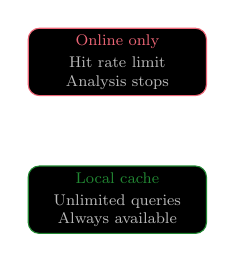
\begin{tikzpicture}[scale=0.7, transform shape,
        box/.style={rounded corners, text width=3cm, align=center, minimum height=1.2cm, font=\footnotesize}
    ]
      % Online-only approach
      \node[box, draw=defconorange, fill=black, text=defconorange] (online) at (0,2)
           {Online only\\[2pt]\textcolor{defcongray}{Hit rate limit\\Analysis stops}};
      % Local cache approach
      \node[box, draw=defcongreen, fill=black, text=defcongreen] (local) at (0,-0.5)
           {Local cache\\[2pt]\textcolor{defcongray}{Unlimited queries\\Always available}};
    \end{tikzpicture}
  \end{columns}
\end{frame}

% This frame addresses LLM-specific availability risks such as API
% quotas, model deprecation, and service outages that can interrupt
% investigations.
\begin{frame}{Availability risk - LLM access}
  \begin{columns}
    \column{0.6\textwidth}
    \begin{itemize}
    \item \textbf{Cloud LLM limitations}
      \begin{itemize}
      \item API rate limits (requests/minute)
      \item Token quotas exhaust quickly
      \item Models deprecated without warning
      \end{itemize}
    \item \textbf{Solution: Local LLMs}
      \begin{itemize}
      \item No API limits
      \item Process entire datasets
      \item Models never disappear
      \end{itemize}
    \end{itemize}
    
    \column{0.4\textwidth}
    \centering
    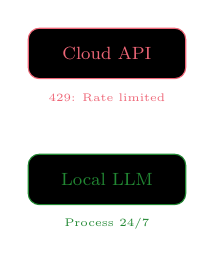
\begin{tikzpicture}[scale=0.8, transform shape,
        box/.style={rounded corners, minimum width=2.5cm, minimum height=0.8cm, font=\footnotesize}
    ]
      % Cloud limits
      \node[box, draw=defconorange, fill=black, text=defconorange] (cloud) at (0,2) {Cloud API};
      \node[text=defconorange, font=\tiny] at (0,1.3) {429: Rate limited};
      
      % Local unlimited
      \node[box, draw=defcongreen, fill=black, text=defcongreen] (local) at (0,0) {Local LLM};
      \node[text=defcongreen, font=\tiny] at (0,-0.7) {Process 24/7};
    \end{tikzpicture}
  \end{columns}
\end{frame}

% The "Methods" section is the solution section. The "OPSEC Risks and
% Challenges" section described the "why" and the problem we are
% solving. This "Methods" section describes the overall approach
% investigators and analysts can use to overcome the problems in the
% previous section. Each step in the "Methods" section should then be
% demonstrated with the example Case Study in the subsequent section.
\section{Methods}

% This is a DEF CON talk and not a commercial vendor talk. This slide
% describes what an individual analyst or investigator can do
% differently to overcome the problems in the previous section. The
% goal is to teach and empower the audience with a new way of
% working. The section is general and in support of the audience
% members selecting their own tools and specific ways of working. The
% code in this project is an example the demonstrates the feasibility
% of the methodology for the specific case study.
\begin{frame}{Methodology: Local Knowledge Graphs}
  \begin{columns}
    \column{0.5\textwidth}
    \begin{itemize}
    \item \textbf{Traditional Approach}
      \begin{itemize}
      \item Query external sources repeatedly
      \item Process with cloud LLMs
      \item Discard after analysis
      \end{itemize}
    \item \textbf{Our Approach}
      \begin{itemize}
      \item Download once, store locally
      \item Process with local LLMs
      \item Build reusable knowledge graph
      \end{itemize}
    \end{itemize}
    
    \column{0.5\textwidth}
    \centering
    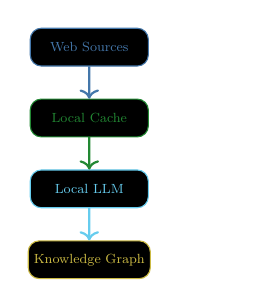
\begin{tikzpicture}[scale=0.6, transform shape,
        box/.style={rounded corners, minimum width=2.5cm, minimum height=0.8cm, text centered,
          font=\footnotesize}]
      % Flow diagram
      \node[box, draw=defconblue, fill=black, text=defconblue] (sources) at (0,3) {Web Sources};
      \node[box, draw=defcongreen, fill=black, text=defcongreen] (cache) at (0,1.5) {Local Cache};
      \node[box, draw=defconcyan, fill=black, text=defconcyan] (llm) at (0,0) {Local LLM};
      \node[box, draw=defconyellow, fill=black, text=defconyellow] (kg) at (0,-1.5) {Knowledge Graph};

      \draw[->, thick, defconblue] (sources) -- (cache);
      \draw[->, thick, defcongreen] (cache) -- (llm);
      \draw[->, thick, defconcyan] (llm) -- (kg);

      \node[text=white, font=\tiny] at (2.5,1.5) {Tor + Browser};
      \node[text=white, font=\tiny] at (2.5,0) {Extract entities};
      \node[text=white, font=\tiny] at (2.5,-1.5) {RDF triples};
    \end{tikzpicture}
  \end{columns}
\end{frame}

% This frame distills the general method into procedural knowledge
% that someone can follow step-by-step. This is the procedure that
% will be followed in the case study. The procedure should show
% specific steps that someone could follow to execute one possible
% implementation of the method. This is more specific than the general
% method but less specific than the case study.
\begin{frame}{Procedure}
  \begin{columns}
    \column{0.7\textwidth}
    \begin{enumerate}
    \item \textbf{Collect Sources}
      \begin{itemize}
      \item Download via Tor
      \item Capture JavaScript content
      \end{itemize}
    \item \textbf{Extract Information}
      \begin{itemize}
      \item Local LLM extraction
      \item Create Resource Description Framework (RDF) triples %verbalize what a triple is
      \end{itemize}
    \item \textbf{Build Knowledge Graph}
      \begin{itemize}
      \item Store in triplestore
      \item Link with ontologies/semantic layers
      \end{itemize}
    \item \textbf{Query \& Analyze}  
      \begin{itemize}
      \item SPARQL queries
      \item GraphRAG insights
      \end{itemize}
    \end{enumerate}

    \column{0.3\textwidth}
    \centering
    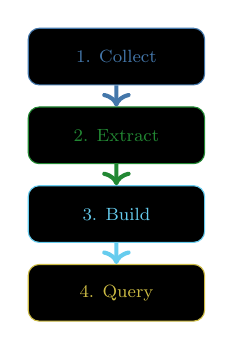
\begin{tikzpicture}[scale=0.8, transform shape,
        box/.style={rounded corners, minimum width=2.8cm, minimum height=0.9cm, text centered, font=\footnotesize}]
      \node[box, draw=defconblue, fill=black, text=defconblue] (s1) at (0,2.5) {1. Collect};
      \node[box, draw=defcongreen, fill=black, text=defcongreen] (s2) at (0,1.25) {2. Extract};
      \node[box, draw=defconcyan, fill=black, text=defconcyan] (s3) at (0,0) {3. Build};
      \node[box, draw=defconyellow, fill=black, text=defconyellow] (s4) at (0,-1.25) {4. Query};

      \draw[->, defconblue, line width=1.5pt] (s1) -- (s2);
      \draw[->, defcongreen, line width=1.5pt] (s2) -- (s3);
      \draw[->, defconcyan, line width=1.5pt] (s3) -- (s4);
    \end{tikzpicture}
  \end{columns}
\end{frame}

% The remainder of the frames in this section describe each step in the
% procedure in more detail. These are specific enough to describe the
% code in the project.
\begin{frame}{Collect Sources}
  \begin{columns}
    \column{0.5\textwidth}
    \begin{itemize}
    \item \textbf{Our implementation}
      \begin{itemize}
      \item Rust + Arti (Tor client)
      \item Playwright + Chromium
      \item Full JavaScript execution
      \item \texttt{collect} CLI tool
      \end{itemize}
    \item \textbf{Why not alternatives?}
      \begin{itemize}
      \item wget/curl: No JavaScript
      \item HTTrack: Incomplete iframes
      \item Direct browser: Exposes IP and cumbersome to script
      \end{itemize}
    \end{itemize}
    
    \column{0.5\textwidth}
    \centering
    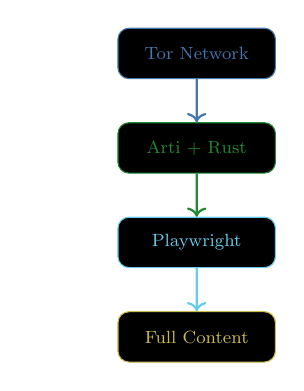
\begin{tikzpicture}[scale=0.8, transform shape,
        box/.style={rectangle, rounded corners, minimum width=2.5cm, minimum height=0.8cm, text centered, font=\footnotesize}]
      % Pipeline
      \node[box, draw=defconblue, fill=black, text=defconblue] (tor) at (0,2) {Tor Network};
      \node[box, draw=defcongreen, fill=black, text=defcongreen] (arti) at (0,0.5) {Arti + Rust};
      \node[box, draw=defconcyan, fill=black, text=defconcyan] (browser) at (0,-1) {Playwright};
      \node[box, draw=defconyellow, fill=black, text=defconyellow] (content) at (0,-2.5) {Full Content};
      
      \draw[->, thick, defconblue] (tor) -- (arti);
      \draw[->, thick, defcongreen] (arti) -- (browser);
      \draw[->, thick, defconcyan] (browser) -- (content);
      
      % Benefits
      \node[text=white, font=\tiny, align=right] at (-2,1.25) {Hide IP};
      \node[text=white, font=\tiny, align=right] at (-2,-0.25) {Control};
      \node[text=white, font=\tiny, align=right] at (-2,-1.75) {JS/iframes};
    \end{tikzpicture}
  \end{columns}
\end{frame}

% This slide describes the next step in the procedure in more detail
% following the pattern of the previous slide.
\begin{frame}{Extract Information}
  \begin{columns}
    \column{0.5\textwidth}
    \begin{itemize}
    \item \textbf{Local LLM extraction}
      \begin{itemize}
      \item No data leaves your system
      \item Process entire datasets
      \item \texttt{enrich} CLI tool
      \end{itemize}
    \item \textbf{What we extract}
      \begin{itemize}
      \item Named entities (people, orgs)
      \item Relationships
      \item Structured JSON/RDF
      \end{itemize}
    \item \textbf{Example: Speakers}
      \begin{itemize}
      \item Input: HTML pages
      \item Output: Speaker + affiliation list JSON
      \end{itemize}
    \end{itemize}
    
    \column{0.5\textwidth}
    \centering
    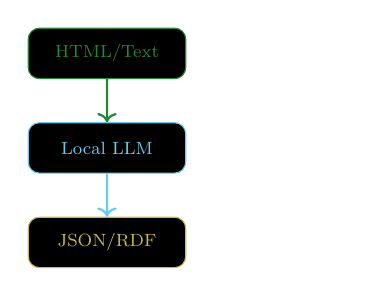
\begin{tikzpicture}[scale=0.8, transform shape,
        box/.style={rectangle, rounded corners, minimum width=2.5cm, minimum height=0.8cm, text centered, font=\footnotesize}]
      % Flow
      \node[box, draw=defcongreen, fill=black, text=defcongreen] (html) at (0,2) {HTML/Text};
      \node[box, draw=defconcyan, fill=black, text=defconcyan] (llm) at (0,0.5) {Local LLM};
      \node[box, draw=defconyellow, fill=black, text=defconyellow] (json) at (0,-1) {JSON/RDF};
      
      \draw[->, thick, defcongreen] (html) -- (llm);
      \draw[->, thick, defconcyan] (llm) -- (json);
      
      % Example
      \node[text=white, font=\tiny, align=left] at (2.5,2) {<div>John Doe</div>};
      \node[text=white, font=\tiny, align=left] at (2.5,-1) {\{"name": "John Doe"\}};
    \end{tikzpicture}
  \end{columns}
\end{frame}

% This slide describes the next step in the procedure in more detail
% following the pattern of the previous slide.
\begin{frame}{Build Knowledge Graph}
  \begin{columns}
    \column{0.5\textwidth}
    \begin{itemize}
    \item \textbf{RDF Triple Store}
      \begin{itemize}
      \item Standard W3C format
      \item Interoperable data
      \end{itemize}
    \item \textbf{Link with ontologies}
      \begin{itemize}
      \item Friend of a Friend (FOAF) for people/orgs
      \item Domain-specific
      \item Enables reasoning
      \end{itemize}
    \item \textbf{Benefits}
      \begin{itemize}
      \item Combine multiple sources
      \item Query across datasets
      \end{itemize}
    \end{itemize}
    
    \column{0.5\textwidth}
    \centering
    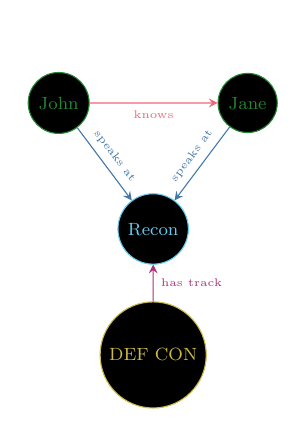
\begin{tikzpicture}[scale=0.8, transform shape,
        node/.style={circle, minimum size=0.8cm, font=\footnotesize},
        edge/.style={->, >=stealth, font=\tiny}]
      % Nodes
      \node[node, draw=defcongreen, fill=black, text=defcongreen] (john) at (0,2) {John};
      \node[node, draw=defcongreen, fill=black, text=defcongreen] (jane) at (3,2) {Jane};
      \node[node, draw=defconcyan, fill=black, text=defconcyan] (recon) at (1.5,0) {Recon};
      \node[node, draw=defconyellow, fill=black, text=defconyellow] (defcon) at (1.5,-2) {DEF CON};
      
      % Edges
      \draw[edge, defconblue] (john) -- node[above, sloped] {speaks at} (recon);
      \draw[edge, defconblue] (jane) -- node[above, sloped] {speaks at} (recon);
      \draw[edge, defconorange] (john) -- node[below, sloped] {knows} (jane);
      \draw[edge, defconpurple] (defcon) -- node[right] {has track} (recon);
      
      % Legend
      \node[text=white, font=\tiny] at (1.5,3) {Knowledge Graph};
    \end{tikzpicture}
  \end{columns}
\end{frame}

% This slide describes the next step in the procedure in more detail
% following the pattern of the previous slide.
\begin{frame}{Query \& Analyze}
  \begin{columns}
    \column{0.5\textwidth}
    \begin{itemize}
    \item \textbf{SPARQL queries}
      \begin{itemize}
      \item Standard query language
      \item Complex relationships
      \item Cross-dataset joins
      \end{itemize}
    \item \textbf{GraphRAG insights}
      \begin{itemize}
      \item Graph-based reasoning
      \item Pattern discovery
      \item Hidden connections
      \end{itemize}
    \item \textbf{Example queries}
      \begin{itemize}
      \item "Who knows whom?"
      \item "Common speakers?"
      \item "Network clusters?"
      \end{itemize}
    \end{itemize}
    
    \column{0.5\textwidth}
    \centering
    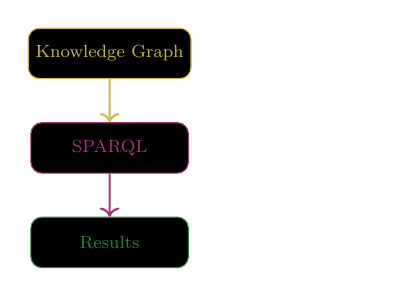
\begin{tikzpicture}[scale=0.8, transform shape,
        box/.style={rectangle, rounded corners, minimum width=2.5cm, minimum height=0.8cm, text centered, font=\footnotesize}]
      % Query flow
      \node[box, draw=defconyellow, fill=black, text=defconyellow] (kg) at (0,2) {Knowledge Graph};
      \node[box, draw=defconpurple, fill=black, text=defconpurple] (sparql) at (0,0.5) {SPARQL};
      \node[box, draw=defcongreen, fill=black, text=defcongreen] (results) at (0,-1) {Results};
      
      \draw[->, thick, defconyellow] (kg) -- (sparql);
      \draw[->, thick, defconpurple] (sparql) -- (results);
      
      % Example query
      \node[text=white, font=\tiny, align=left] at (2.7,0.5) {SELECT ?person\\WHERE \{\\  ?person :speaks\_at Recon .\\  ?person :knows ?other\\\}};
    \end{tikzpicture}
  \end{columns}
\end{frame}

% This section illustrates the manual approach of analyzing the
% speakers at this year's Recon Village. This section provides a
% baseline of how an individual investigator might approach the
% investigation with traditional tools. We will use this baseline to
% demonstrate the advantages of our method and procedure.
\section{Case Study - Traditional Approach}

% This frame shows how the current Recon Village website presents
% content that lists the speakers and the schedule. The presentation
% will highlight that with sufficient effort the technical content can
% be reverse engineered and parsed however doing so depends on
% computer programming skills rather than investigative skills. This
% website uses JavaScript to render content dynamically and iframes
% for content. Therefore, simple scraping tools fail to capture all of
% the content of interest in the file they output. In addition, even
% interactively using a web browser with CTRL+F to find names will
% fail if they are on Friday vs Saturday, since the iframe for the
% schedule only renders one of those pages at a time.
%
% The Recon Village schedule is also available as a structured source
% from Sessionize (\url{https://sessionize.com}). DEF CON web and
% Hacker Tracker data is available in a Firebase. This is just
% illustrative for the method and not a criticism of the website. Many
% modern websites exhibit the same technical characteristics.
%
% It is notable that there is JSON-LD, an RDF serialization format, in
% the Recon Village website as well.
\begin{frame}{Target of Investigation: Recon Village 2025}
  Read website with eyeballs. Click things.
  
  \adjustbox{valign=m}{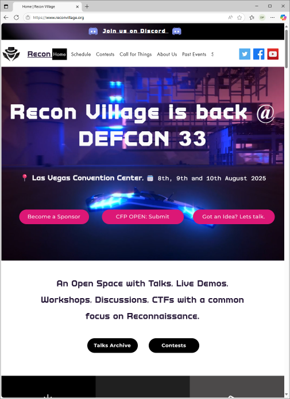
\includegraphics[width=0.225\textwidth]{recon-village-home-page.png}}
  \hfill
  \adjustbox{valign=m}{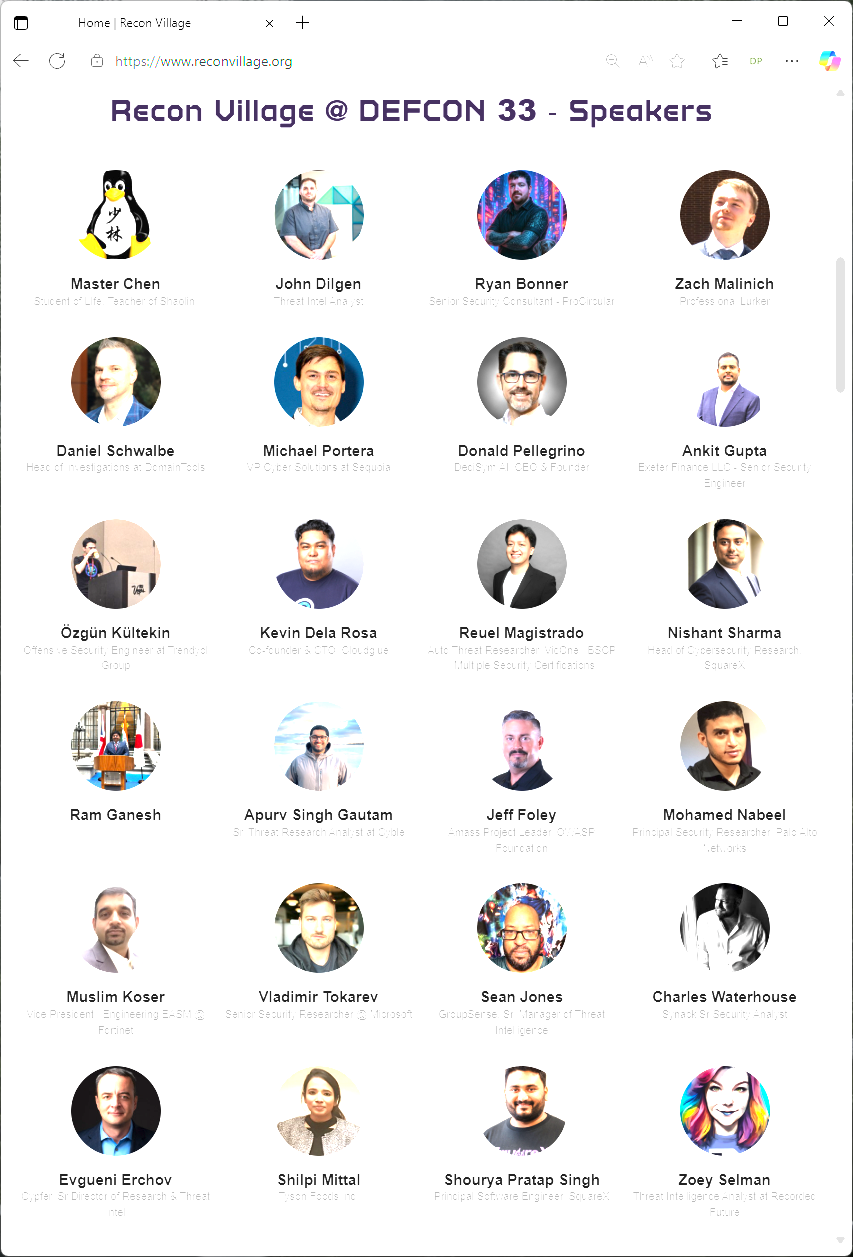
\includegraphics[width=0.225\textwidth]{2025-08-03-153751-speaker-block.png}}
  \hfill
  \adjustbox{valign=m}{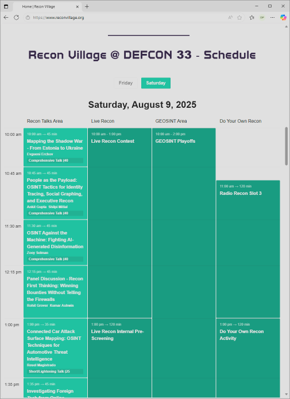
\includegraphics[width=0.225\textwidth]{recon-village-schedule-iframe.png}}  
\end{frame}

\begin{frame}{Manual Sociogram}
  \begin{columns}[c]
    \column{0.6\textwidth}
    \centering
    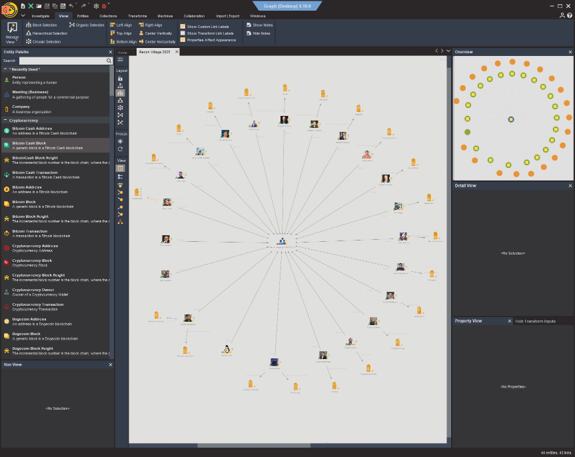
\includegraphics[height=0.8\textheight]{maltego-manual-sociogram.png}
    
    \column{0.4\textwidth} Manual data reduction and transformation by
    reading browser rendering and clicking on Graphical User Interface
    (GUI).
  \end{columns}
\end{frame}

\section{Case Study - Demo}

\subsection{collect}

\begin{frame}{Automated Collection}
  Challenge: ``wget –-mirror'' speaker and schedule information missing due
  to use of <iframe> and JavaScript.
  \begin{tikzpicture}[
      node distance=3cm,
      block/.style={inner sep=0pt},
      arrow/.style={->, >=Stealth, thick, color=defconcyan}
    ]

    \node[block] (tor) {
\includegraphics[width=2cm]{tor-logo.png}};
    \node[block, right of=tor] (arti) {
\includegraphics[width=2cm]{arti-logo.png}};
    \node[block, right of=arti] (rust) {
\includegraphics[width=2cm]{rust-logo.png}};
    \node[block, right of=rust] (playwright) {
\includegraphics[width=2cm]{playwright-logo.png}};
    \node[block, right of=playwright] (chromium) {
\includegraphics[width=2cm]{chromium-logo.png}};

    \draw[arrow] (tor) -- (arti);
    \draw[arrow] (arti) -- (rust);
    \draw[arrow] (rust) -- (playwright);
    \draw[arrow] (playwright) -- (chromium);
  \end{tikzpicture}
\end{frame}

% The purpose of this frame is to highlight remaining risks and
% limitations. The method improves over some current practices but
% many challenges remain. Avoid giving the incorrect impression that
% the method is a silver bullet. Risk: Don't trust Chromium being run
% by Playwright.
\begin{frame}{Automated Collection Risks and Limitations}
  \begin{itemize}
  \item The web browser may generate unexpected network traffic over Tor
  \item Browser fingerprinting can still occur despite Tor usage
  \item Tor exit nodes may log or modify traffic
  \item Performance limitations: Tor + browser automation is slower
  \item Some sites detect and block automated browsers
  \item J. Schmetz, "Your privacy on Chrome is at risk, here's what
    you can do," \textit{TechRadar}, Oct. 08, 2024.
  \end{itemize}
\end{frame}

\begin{frame}{collect CLI}
  \centering
  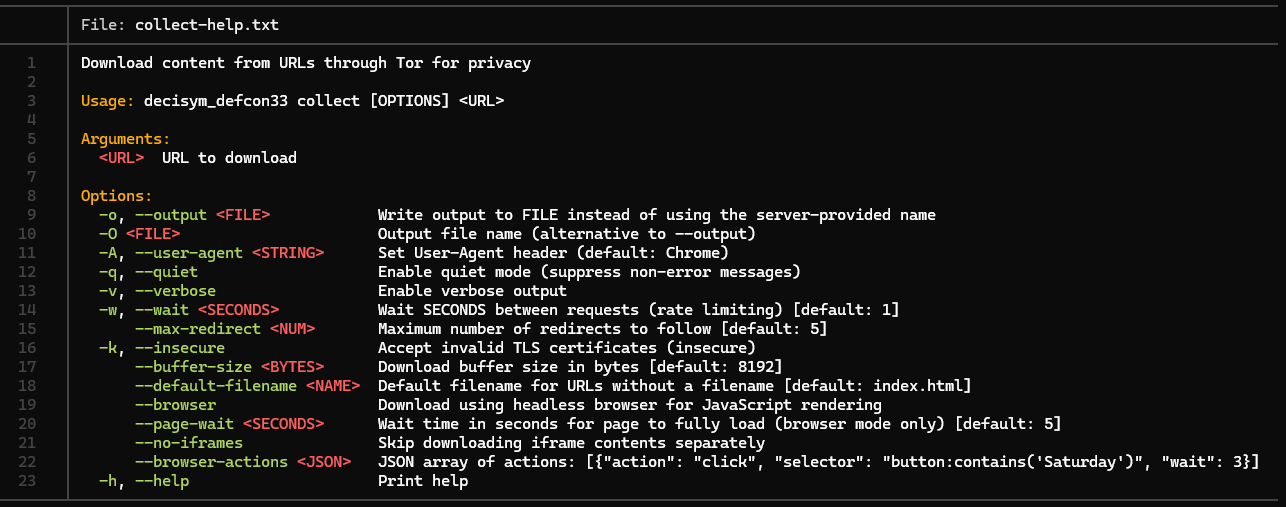
\includegraphics[height=0.75\textheight]{collect-help.png}
\end{frame}

\subsection{enrich}

\begin{frame}{Salient Information Extraction}
  \begin{itemize}
  \item \textbf{Found by LLM, missed by human:}
    \begin{itemize}
    \item Sinwindie
    \item Kumar Ashwin
    \item Rohit Grover
    \item Kaloyan Ivanov
    \end{itemize}
  \item \textbf{Why manual search failed:}
    \begin{itemize}
    \item CTRL+F didn't work
    \item Hidden in Saturday iframe
    \item Not in main speaker grid
    \end{itemize}
  \end{itemize}
\end{frame}

% This frame shows a visualizations of some of the entities in the
% FOAF ontology as a graph.
% http://ontology.tib.eu/educor/visualization
% http://xmlns.com/foaf/spec/
\begin{frame}{Friend of a Friend (FOAF) Ontology}
  \centering
  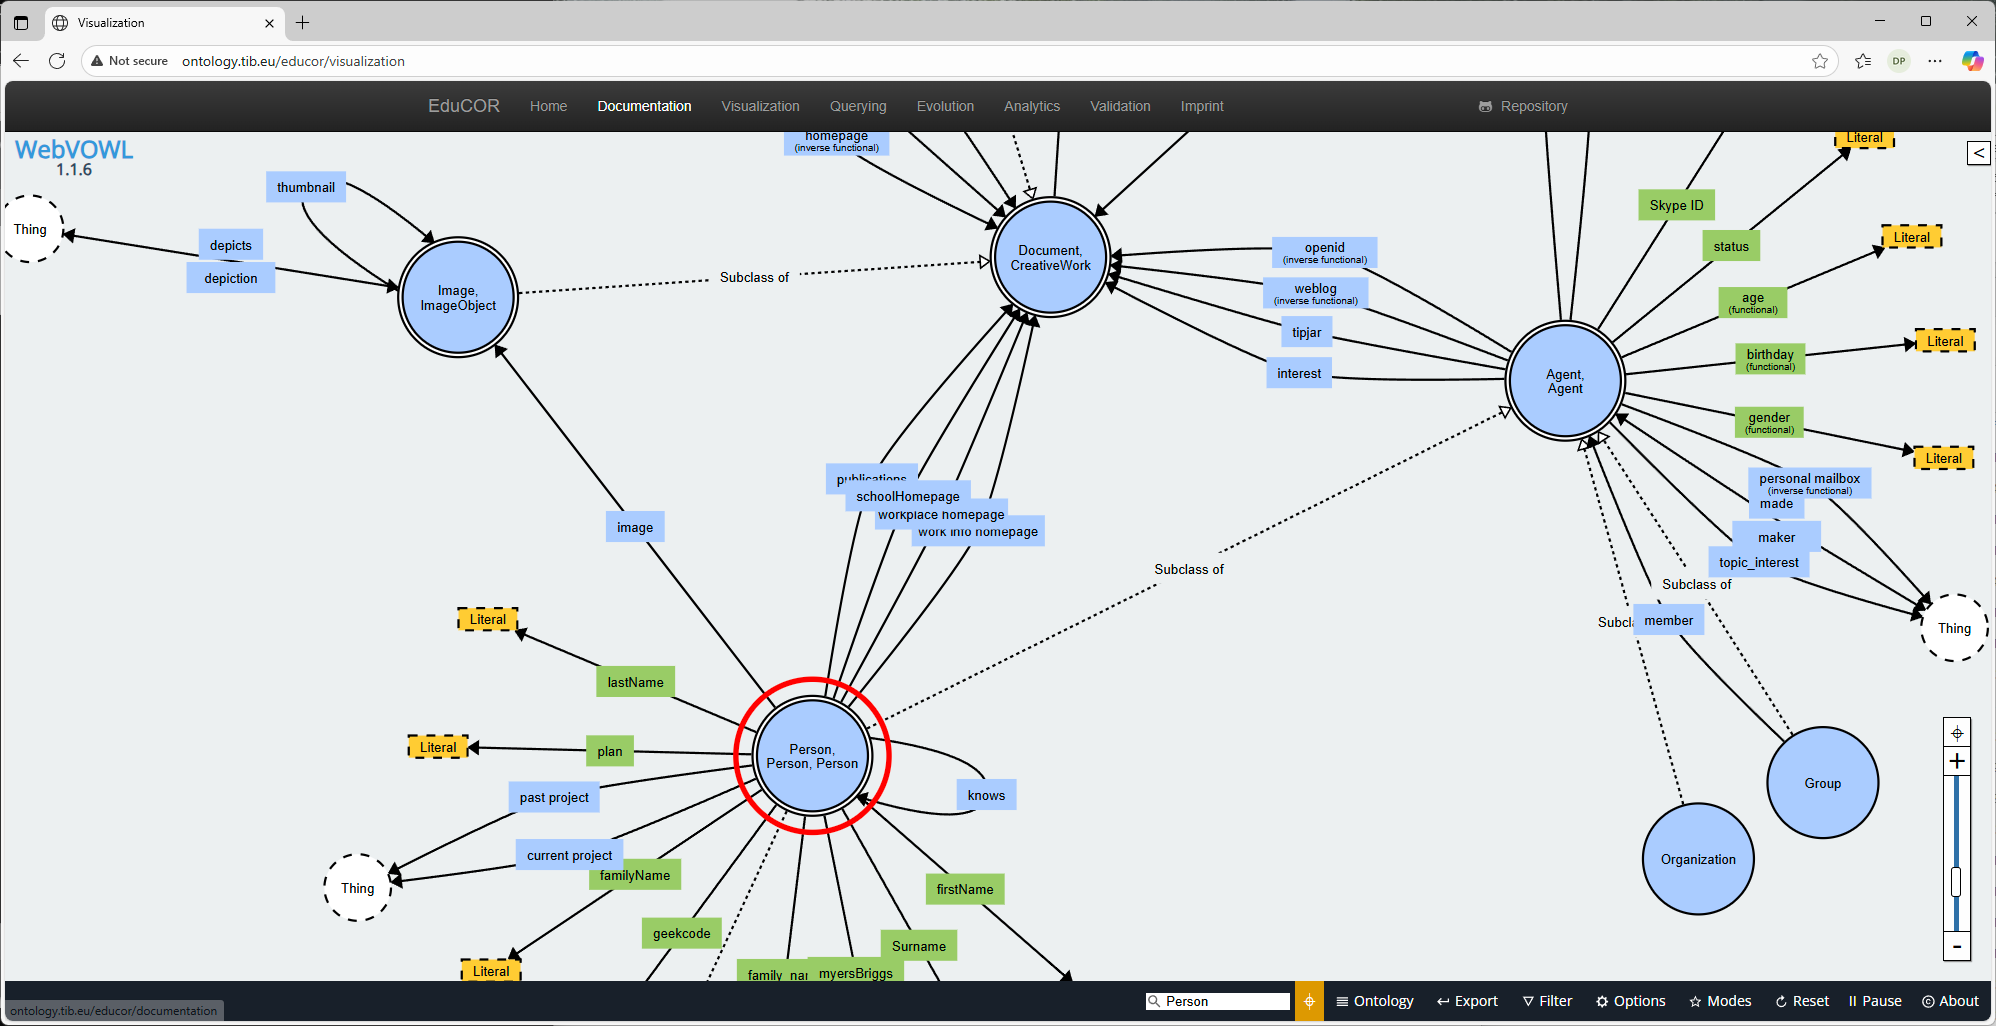
\includegraphics[height=0.75\textheight]{foaf-person-webvowl.png} 
\end{frame}

% This frame shows the color-syntax highlighted output of `batcat`
% over the YAML template used to prompt the LLM to generate RDF
% aligned to OWL.
\begin{frame}{Generate RDF, align to FOAF ontology}
  \centering
  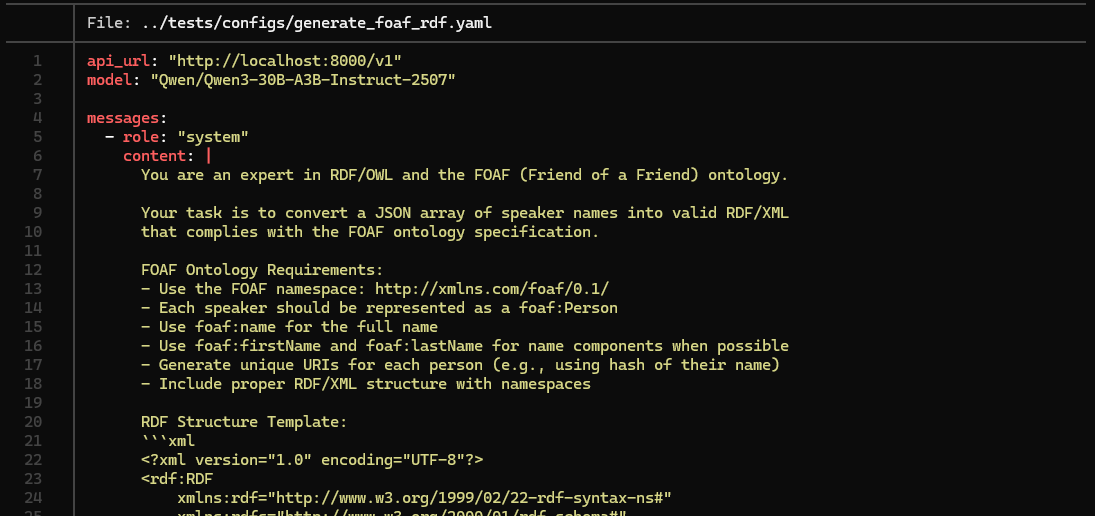
\includegraphics[height=0.75\textheight]{generate_foaf_rdf.png}
\end{frame}

% This frame shows the results of linking speaker data with Wikidata
% to analyze company founding dates and industry classifications
\begin{frame}{Knowledge Graph Integration: Speaker Company Analysis}
  \begin{columns}[c]
    \column{0.55\textwidth}
    \begin{itemize}
    \item \textbf{Linked FOAF to Wikidata}
      \begin{itemize}
      \item 28 speakers extracted
      \item 7 companies matched in Wikidata
      \item Founded 1935-2012
      \end{itemize}
    \item \textbf{Industry Distribution}
      \begin{itemize}
      \item Computer Security: 3
      \item Information Technology: 2
      \item Cybersecurity: 1
      \item Agriculture: 1
      \end{itemize}
    \item \textbf{Key Insight}: Mix of established companies (Microsoft, 50 years) and newer security firms (Synack, 13 years)
    \end{itemize}
    
    \column{0.45\textwidth}
    \small
    \begin{tabular}{lr}
      \hline
      \textbf{Company} & \textbf{Age} \\
      \hline
      Tyson Foods & 90 years \\
      Microsoft & 50 years \\
      Fortinet & 25 years \\
      OWASP & 24 years \\
      Palo Alto Networks & 20 years \\
      Recorded Future & 17 years \\
      Synack & 13 years \\
      \hline
    \end{tabular}
  \end{columns}
\end{frame}

% This frame shows the results of linking speaker data with a variety
% of company info found on the web and then building an Automaton dashboard
\begin{frame}{Knowledge Graph Integration: Dashboard}
  \centering
  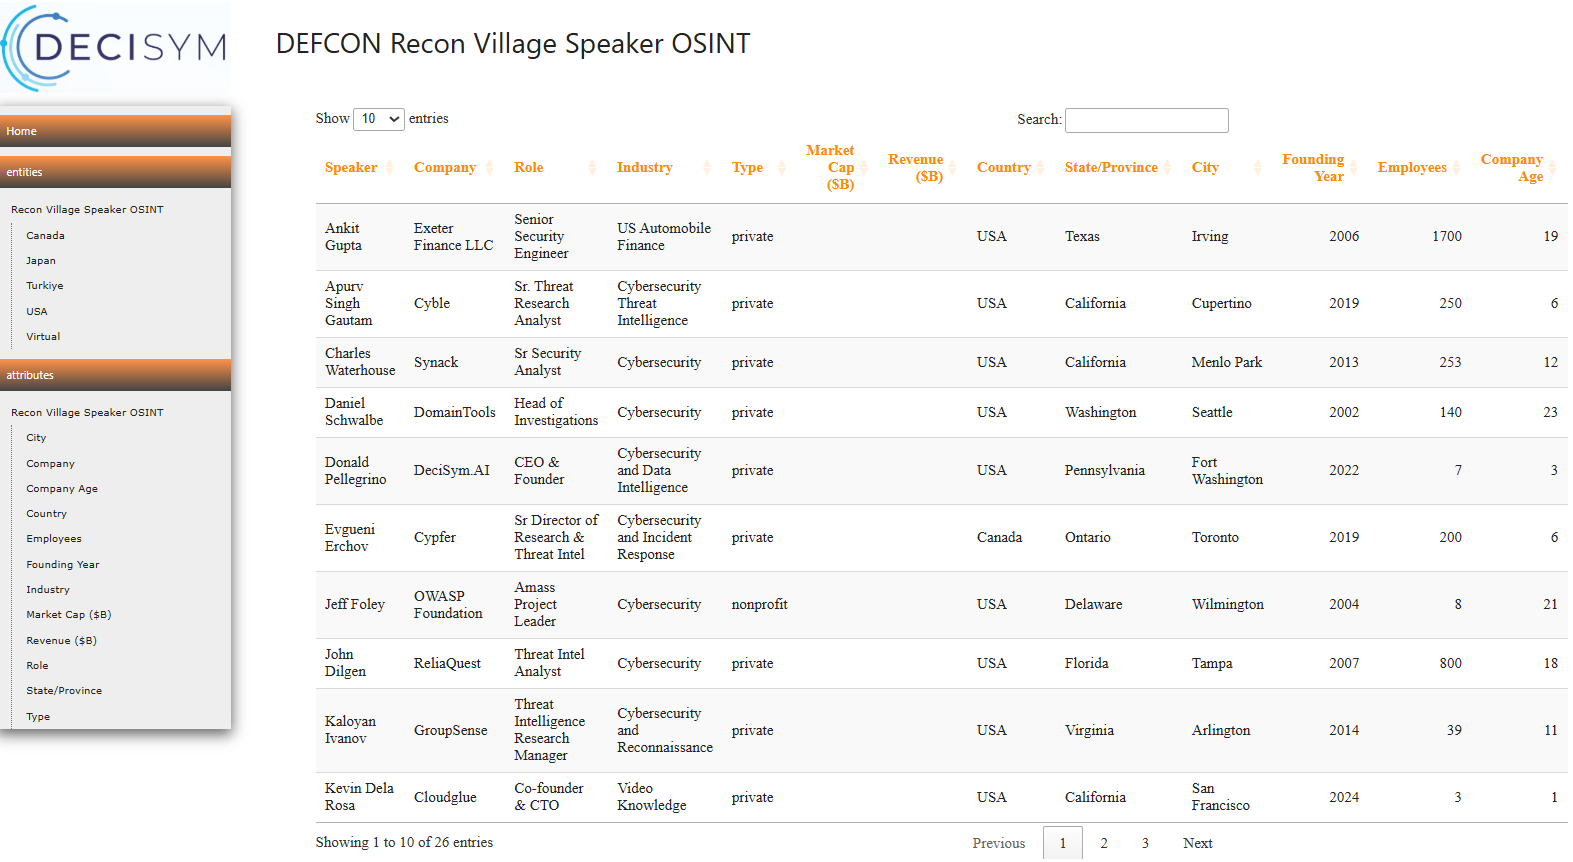
\includegraphics[height=0.75\textheight]{automaton_snapshot_2025-08-06.png}
\end{frame}

\section{Summary}

\begin{frame}{Stack}
  \begin{itemize}
  \item User decisions
    \begin{itemize}
    \item Source selection (e.g., websites)
    \item Salient feature identification (e.g., Speakers)
    \item Ontology selection (e.g., FOAF)
    \end{itemize}
  \item Tools
    \begin{itemize}
    \item Workflow support (e.g., scripts, DeciSym.AI Engine, LM Studio)
    \item Crawlers (e.g., Tor Arti)
    \item Triplestore (e.g., DeciSym.AI Engine, Oxigraph)
    \end{itemize}
  \item LLM
    \begin{itemize}
    \item Model (e.g., Qwen3-30B-A3B-Instruct-2507)
    \item Runtime (e.g., vLLM, Docker image rocm/vllm)
    \end{itemize}
  \item Linux Distribution (e.g., Ubuntu 24.04.2 LTS)
  \item Hardware (e.g., AMD or Nvidia GPU)
  \end{itemize}
\end{frame}

\begin{frame}{Summary}
  \begin{itemize}
  \item Bypass LLM rate limits by building a local cache of sources over time.    
    \begin{itemize}
    \item Sources can be reused and shared
    \item Sources can be integrated
    \end{itemize}
  \item Maintain OPSEC by working on local cache.
  \item Enable scientific repeatability and reusability with workflow management.
  \end{itemize}
\end{frame}

% Bypass rate limits by building a local cache of sources over time.

% Maintain OPSEC by working on the local cache.

% Enable scientific repeatability with metadata and workflow
% management.

\begin{frame}{Contacts}
  \begin{itemize}
  \item Recon Village: \url{https://www.reconvillage.org}
  \item Supplementary Materials: \url{https://github.com/DeciSym}
  \item Email: \url{don@decisym.ai}
  \end{itemize}
  \tikz[remember picture,overlay] {
  \node[xshift=12.5cm,yshift=1.3cm]
  {
\includegraphics[width=2.5cm,clip]{don_pellegrino_vcard_qr_code.png}};
  }
\end{frame}

\end{document}
